% 
% Annual Cognitive Science Conference
% Sample LaTeX Paper -- Proceedings Format
% 

% Original : Ashwin Ram (ashwin@cc.gatech.edu)       04/01/1994
% Modified : Johanna Moore (jmoore@cs.pitt.edu)      03/17/1995
% Modified : David Noelle (noelle@ucsd.edu)          03/15/1996
% Modified : Pat Langley (langley@cs.stanford.edu)   01/26/1997
% Latex2e corrections by Ramin Charles Nakisa        01/28/1997 
% Modified : Tina Eliassi-Rad (eliassi@cs.wisc.edu)  01/31/1998
% Modified : Trisha Yannuzzi (trisha@ircs.upenn.edu) 12/28/1999 (in process)
% Modified : Mary Ellen Foster (M.E.Foster@ed.ac.uk) 12/11/2000
% Modified : Ken Forbus                              01/23/2004
% Modified : Eli M. Silk (esilk@pitt.edu)            05/24/2005
% Modified : Niels Taatgen (taatgen@cmu.edu)         10/24/2006
% Modified : David Noelle (dnoelle@ucmerced.edu)     11/19/2014

%% Change "letterpaper" in the following line to "a4paper" if you must.

\documentclass[10pt,letterpaper]{article}

\usepackage{cogsci}
\usepackage{pslatex}
\usepackage{apacite}

\usepackage{amsmath}
\usepackage{graphicx}
\usepackage{subcaption}

% http://tex.stackexchange.com/questions/205342/issues-with-flushend-last-citation-cut-etc 
\usepackage[keeplastbox]{flushend}  % balance the final columns

\renewcommand{\vec}[1]{{\bf {#1}}}
\newcommand{\dotp}[3]{\left\langle {#1}, {#2} \right\rangle_{#3}}
\newcommand{\lif}[2]{G_{#1} \left[ {#2} \right]}

\title{A Spiking Neural Bayesian Model of Life Span Inference}
 
\author{{\large \bf Sugandha Sharma (s72sharm@uwaterloo.ca)} \\
  {\large \bf Aaron R. Voelker (arvoelke@uwaterloo.ca)} \\
  {\large \bf Chris Eliasmith (celiasmith@uwaterloo.ca)} \\
  Centre for Theoretical Neuroscience, University of Waterloo \\
  Waterloo, ON, Canada, N2L 3G1}


\begin{document}

\maketitle

\begin{abstract}
In this paper, we present a spiking neural model of life span inference. Through this model, we explore the biological plausibility of performing Bayesian computations in the brain. Specifically, we address the issue of representing probability distributions using neural circuits and combining them in meaningful ways to perform inference.  We show that applying these methods to the life span inference task matches human performance on this task better than an ideal Bayesian model due to the use of neuron tuning curves.  We also describe potential ways in which humans might be generating the priors needed for this inference. This provides an initial step towards better understanding how Bayesian computations may be implemented in a biologically plausible neural network. 

\textbf{Keywords:} 
Neural Engineering Framework; biologically plausible inference; neural bayesian model; expectation maximization 
\end{abstract}

\section{Introduction}

Computations performed by the nervous system are subject to uncertainty because of the influence of sensory, cellular, and synaptic noise. At the level of cognition, the models that the brain uses to interact with its environment must necessarily cope with missing and imperfect information about the world. Behavioral studies have confirmed that humans often account for uncertainty in a way that is nearly optimal in the Bayesian sense~(i.e.,~``Bayes optimal'')~\cite{ma2006bayesian}). This implies that (1) neural circuits must, at least implicitly, represent probability distributions, and (2) neural circuits must be able to effectively compute with these probability distributions in order to perform Bayesian inference near-optimally. 

Probabilistic models based on Bayes' rule have been widely used for understanding human cognition including inference, parameter and structure learning~\cite{jacobs2011bayesian}, and word learning~\cite{xu2007word}. However, most Bayesian models lack biological plausibility because it is unclear how these computations might be realized in the brain. In particular, these models rely on sophisticated computations including high-dimensional integration, precise multiplication, and large-scale structure representation, without the use of spiking neuron models to implement these necessary computations.

A biologically plausible Bayesian approach can provide us insights into the working of the brain at multiple levels of analysis~\cite{eliasmith2013build}. Moreover, it can also help in making more accurate normative predictions about how the perceptual system combines prior knowledge with sensory observations, enabling more accurate interpretations of data from psychological experiments~\cite{doya2007bayesian}.  And finally, it can point the way towards approximate Bayesian algorithms that are efficiently implemented in a neural substrate.

\citeA{griffiths2012bayesians} conclude that different theoretical frameworks, such as Bayesian modeling and connectionism, have different insights to offer about human cognition, distributed across different levels of analysis. Here we make an initial attempt towards integrating these frameworks. We explore the biological plausibility of Bayesian inference by implementing a neural model of a life span prediction task using the Neural Engineering Framework~\cite<NEF;>{eliasmith2003neural}. We answer questions about how probability distributions can be represented in a connectionist framework using spiking neurons, and how the neural representations of these probability distributions can be used in meaningful ways. The next section describes the life span prediction task which we use.

\section{Life span prediction task}

\citeA{griffiths2006optimal} evaluate how cognitive judgments compare with optimal statistical inference by asking people to predict human life spans. A group of 208 people were asked to predict human life spans, after being presented by a question in survey format as given below:

``Insurance agencies employ actuaries to make predictions about people's life spans -- the age at which they will die based upon demographic information. If you were assessing an insurance case for an 18-year-old man, what would you predict for his life span?"

The responses were recorded and compared with the predictions made by a Bayesian model.

\subsection{Bayesian model}

If $t_{total}$ indicates the total amount of time the person will live and $t$ indicates his current age, the task is to estimate $t_{total}$ from $t$. The Bayesian model computes a probability distribution over $t_{total}$ given $t$, by applying Bayes' rule:
\begin{equation}
\label{eqn:bayes_rule}
\begin{aligned}
p(t_{total} | t) = p(t | t_{total})p(t_{total}) / p(t) ,
\end{aligned}
\end{equation}
where:
\begin{equation}
\label{eqn:p_t}
\begin{aligned}
p(t) = \int_{0}^\infty p(t | t_{total})p(t_{total}) \, dt_{total} .
\end{aligned}
\end{equation}

We assume that the maximum age is $120$ years. 
Thus, when calculating $p(t)$ in practice, the integral may be computed from 0 to 120.

\paragraph{Prior} \citeA{griffiths2006optimal} use publicly available real-world data to identify the true prior distribution $p(t_{total})$ over life spans (shown in Figure~\ref{fig:model_prior_prediction}A).

\paragraph{Likelihood}

The likelihood $p(t | t_{total})$ is the probability of encountering a person at age $t$ given that their total life span is $t_{total}$. \citeA{griffiths2006optimal} assume for simplicity that we are equally likely to meet a person at any point in his or her life. As a result, this probability is uniform, $p(t | t_{total}) = 1/t_{total}$, for all $t < t_{total}$ (and 0 for $t \ge t_{total}$).

\paragraph{Prediction function}

Combining the prior with the likelihood according to Equation~\ref{eqn:bayes_rule} yields a probability distribution $p(t_{total} | t)$ over all possible life spans $t_{total}$ for a person encountered at age $t$. As is standard in Bayesian prediction, \citeA{griffiths2006optimal} use the median of this distribution---the point at which it is equally likely that the true life span is either longer or shorter---as the estimate for $t_{total}$.  This identifies a prediction function that specifies a predicted value of $t_{total}$ for each observed value of $t$. 

\paragraph{Results}

Results obtained by \citeA{griffiths2006optimal} through this Bayesian model are shown in Figure~\ref{fig:model_prior_prediction}B. 


\begin{figure}[h]
\begin{center}
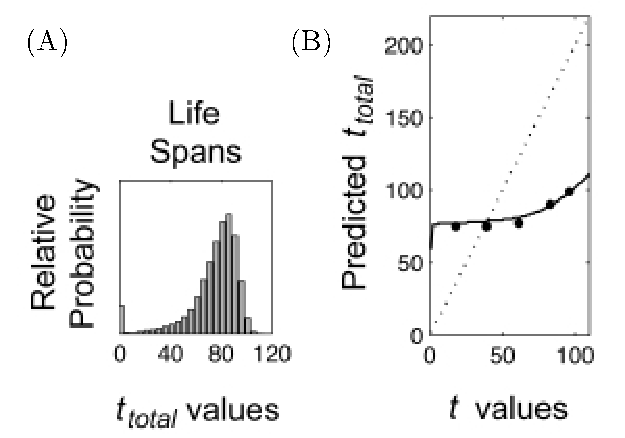
\includegraphics[width=\linewidth, keepaspectratio]{n_prior_prediction.pdf}
\end{center}
\caption{(A) Empirical distribution of the total life span $t_{total}$. (B) Participants' predicted values of $t_{total}$ for a single observed sample $t$. Black dots show the participants' median predictions for $t_{total}$. Solid line shows the optimal Bayesian predictions based on the empirical prior distribution shown in A. Dotted lines show predictions based on a fixed uninformative prior. Note: the fit between the human predictions (black dots) and Bayesian predictions (solid line) looks spot on in this figure due to the compressed y-axis, but Figure~\ref{fig:model_comparison}b shows a zoomed version revealing that this is not the case. Adapted from \citeA{griffiths2006optimal}.} 
\label{fig:model_prior_prediction}
\end{figure}


\section{Neural Engineering Framework}

The Neural Engineering Framework~(NEF) is based on three principles---representation, transformation, and dynamics---which are used to construct large-scale neural models. The first two principles are described in the following sections. The principle of representation also describes how probability distributions can be represented using spiking neurons. The third principle is not required for this paper, and its details can be found elsewhere~\cite{eliasmith2003neural}. 

\subsection{Principle 1 -- Representation}
In the NEF, information is represented as time-varying vectors of real numbers by populations of neurons. We say that a population of neurons has activities $a_i(\vec{x})$, which encode an $n$-dimensional stimulus vector, $\vec{x} = \left[ x_1, x_2, \ldots, x_n \right]$, by defining the encoding:
\begin{equation}
\label{eqn:encoding}
\begin{aligned}
a_i(\vec{x}) = \lif{i}{J_i(\vec{x})}, 
\end{aligned}
\end{equation}
where $\lif{i}{\cdot}$ is the nonlinear transfer function describing the neuron's spiking response, and $J_i(\vec{x})$ is the current entering the soma of the neuron. For the purpose of our model, we have chosen $\lif{i}{\cdot}$ to be the leaky integrate-and-fire~(LIF) neuron model. The soma current is defined by:
\begin{equation}
\label{eqn:current}
\begin{aligned}
J_i(\vec{x}) = \alpha_i \dotp{\vec{e}_i}{\vec{x}}{n} + J_i^{bias} ,
\end{aligned}
\end{equation}
where $J_i(\vec{x})$ is the current in the soma, $\alpha_i$ is a gain and conversion factor, $\vec{x}$ is the stimulus vector to be encoded, $\vec{e}_i$ is the encoding vector which corresponds to the ``preferred stimulus'' of the neuron---consistent with the standard idea of a preferred direction vector~\cite{schwartz1988primate}---and $J_i^{bias}$ is a bias current that accounts for background activity. The notation $\dotp{\cdot}{\cdot}{n}$ indicates an $n$-dimensional dot-product.

Given this encoding, the original stimulus vector can be estimated by decoding those activities as follows:
\begin{equation}
\label{eqn:decoding}
\begin{aligned}
\hat{\vec{x}} = \sum_i a_i(\vec{x}) \vec{d}_i .
\end{aligned}
\end{equation}

The decoding vectors $\vec{d}_i$ (also known as ``representational decoders'') are typically found in the NEF by least-squares optimization, which we use here~\cite{eliasmith2003neural}. Thus, the decoders resulting from this optimization complete the definition of a \textit{population code} over a set of neurons $i$ for the representation of $\vec{x}$. The code is defined by the combination of nonlinear encoding in Eq.~\ref{eqn:encoding} and weighted linear decoding in Eq.~\ref{eqn:decoding}.

\subsubsection{Temporal representation} %\hfill \break
The population code does not explicitly address the issue of how information is encoded over time. To do so, we can begin by considering the temporal code for each neuron in isolation by taking the neural activities to be filtered spike trains as shown in Eq.~\ref{eqn:temp_decoding}:
\begin{equation}
\label{eqn:temp_decoding}
\begin{aligned}
a_i(t) = \sum_m h_i(t) \ast \delta(t-t_m) = \sum_m h_i(t-t_m) ,
\end{aligned}
\end{equation}
where $\delta_i(\cdot)$ are the spikes at time $t_m$ for a given neuron $i$, generated by $\lif{i}{\cdot}$ and $h_i(t)$ are the linear decoding filters. We can compute the optimal filters for decoding using the NEF, however to make our model biologically plausible, we have chosen these filters ($h_i(t)$) to be the postsynaptic currents (PSCs) induced in subsequent neuron by the arrival of a spike. \citeA{eliasmith2003neural} have shown that this assumption causes minimal information loss which can be further reduced by increasing the population size. 

This temporal code can be combined with the population code defined before (Eqs.~\ref{eqn:encoding},~\ref{eqn:current}, \ref{eqn:decoding}), to provide a general \textit{population temporal code} for vectors. The encoding and decoding equations for such a code are given by Eq.~\ref{eqn:encoding_poptemp} and Eq.~\ref{eqn:decoding_poptemp}:
\begin{align}
\delta(t-t_{im}) &= \lif{i}{\alpha_i \dotp{\vec{e}_i}{\vec{x}}{n} + J_i^{bias}} \label{eqn:encoding_poptemp} \\
\hat{\vec{x}} &= \sum_{i,m} h_i(t-t_m) \vec{d}_i . \label{eqn:decoding_poptemp}
\end{align}

\subsubsection{Representing probability distributions}
%\hfill \break
Probability distributions are essentially functions of some parameters. Having described how to represent vectors using the NEF, we consider the relationship between vector and function representation. For any representation, we need to specify the domain of that representation. In case of vectors, the domain is the subspace of the vector space that is represented by the neurons (e.g., the $\vec{x}$ vector). We define the relevant function domain by parameterizing the set of represented functions by an $n$-dimensional vector of coefficients $\vec{k} = \left[ k_1, k_2, \ldots, k_n \right]$. These define any function of interest over a fixed set of basis functions $\phi(\upsilon)$ as follows:
\begin{equation}
\label{eqn:function}
\begin{aligned} 
\vec{x}(\upsilon; \vec{k}) = \sum_{j=1}^n k_j \phi_j(\upsilon)  &, \quad \text{for $k \sim p(\vec{k})$} .
\end{aligned}
\end{equation}
Thus we define a particular probability distribution $p(\vec{k})$ by limiting the space spanned by the basis $\phi(\upsilon)$ to some subspace of interest depending on the application.

This is also the domain over which the optimization to find the decoders in Eq.~\ref{eqn:decoding} is performed. 
 
Next, we define population encoding and decoding analogous to that in Eqs~\ref{eqn:encoding} and \ref{eqn:decoding} for functions:
\begin{align} 
a_i(\vec{x}(\upsilon; \vec{k})) = a_i(\vec{k}) &= \lif{i}{\alpha_i \dotp{\vec{e}_i(\upsilon)} {\vec{x}(\upsilon; \vec{k})}{n} + J_i^{bias}} \label{eqn:function_encoding} \\
%&\text{Decoding:  } \ &&\textbf{\^x}(v; \textbf{k}) = \sum_i a_i(k)d_i(v)
\hat{\vec{x}}(\upsilon; \vec{k}) &= \sum_i a_i(\vec{k})\vec{d}_i(\upsilon), \label{eqn:function_decoding}
\end{align}
where $\vec{e}_i(\upsilon)$ and $\vec{d}_i(\upsilon)$ are the encoding and decoding functions of the neurons. We project these functions onto the same basis $\phi(\upsilon)$ used to identify the function space. For simplicity, we assume that $\phi(\upsilon)$ is an orthonormal basis -- an analogous derivation for a bi-orthonormal set can be found elsewhere~\cite{eliasmith2011normalization}. Hence, we get the following encoding and decoding functions:
\begin{align}
\vec{e}_i(\upsilon) &= \sum_{j=1}^n e_{ij} \phi_j(\upsilon) \label{eqn:encoding_function} \\
\vec{d}_i(\upsilon) &= \sum_{j=1}^n d_{ij} \phi_j(\upsilon), \label{eqn:decoding_function}
\end{align}
% SS-hack
\vspace{-12pt}
where $e_{ij}$ and $d_{ij}$ identify the $n$ coefficients that represent the encoding and decoding functions in $\phi(\upsilon)$ basis for each neuron. We now substitute these into Eq~\ref{eqn:function_encoding}:


%SS-hack
\vspace{-10pt}
\begin{equation}
\label{eqn:final_func_encoding}
\begin{aligned}
a_i(\vec{x}(\upsilon; \vec{k})) & = \lif{i}{\alpha_i\bigg(\sum_{m,n} k_n \phi_n(\upsilon) e_{im} \phi_m(\upsilon)\bigg) +  J_i^{bias}} \\
& = \lif{i}{\alpha_i\bigg(\sum_{m,n} k_n e_{im} \delta_{mn} \bigg) +  J_i^{bias}} \\ 
& = \lif{i}{\alpha_i\bigg(\sum_{n} k_n e_{in} \bigg) +  J_i^{bias}} \\
& = \lif{i}{\alpha_i \dotp{\vec{e}_i}{\vec{k}}{n} +  J_i^{bias}} .
\end{aligned}
\end{equation}


This way, function encoding is expressed as vector encoding identical to Eq.~\ref{eqn:encoding_poptemp}. Similarly, function decoding can also be expressed as vector decoding as follows:
\begin{equation}
\label{eqn:final_func_decoding}
\begin{aligned} 
\hat{\vec{k}} = \sum_i a_i(\vec{k}) \vec{d}_i .
\end{aligned}
\end{equation}

To summarize, we have shown that it is mathematically equivalent to talk in terms of (finite-dimensional) function spaces or (finite-dimensional) vector spaces. Since probability distributions are most generally functions, we can approximate them as high-dimensional vectors over a fixed set of basis functions using the NEF.

\subsection{Principle 2 -- Transformation}
Transformations of neural representations are functions of the vector variables represented by neural populations. 

To perform a transformation $f(\vec{x})$ in the NEF, instead of finding the representational decoders $\vec{d}_i$ to extract the originally encoded variable $\vec{x}$, we can re-weight the decoding to specify some function $f(\vec{x})$ other than identity. In other words, we can find the decoders $\vec{d}_i^{f(\vec{x})}$ (also known as ``transformational decoders'') by using least-squares optimization to minimize the difference between the decoded estimate of $f(\vec{x})$ and the actual $f(\vec{x})$, which results in the transformation:
\begin{equation}
\label{eqn:decoding_transform}
\begin{aligned}
\hat{\vec{x}} = \sum_i a_i(\vec{x})\vec{d}_i^{f(\vec{x})} .
\end{aligned}
\end{equation}

Both linear and nonlinear functions of the encoded vector variable can be computed in this manner~\cite{eliasmith2003neural}. In the NEF, connection weights between neurons can be defined in terms of encoders and decoders as: $\omega_{ij} = \alpha_j \vec{e}_j \vec{d}_i^{f(\vec{x})}$, where $i$ indexes the presynaptic population, $j$ indexes the postsynaptic population, and $\vec{d}_i^{f(\vec{x})}$ are representational or transformational decoders.


% Model Diagram
\begin{figure}[h]
\begin{center}
\includegraphics[width=\linewidth, keepaspectratio]{final_model.png}
\end{center}
\caption{A schematic diagram of the neural model. Here ``Likelihood" and ``Prior'' contain 200 neurons each, ``Product'' network contains 4000 neurons and ``Normalized Posterior" contains 800 neurons.}
\label{fig:final_model}
\end{figure}

\section{Neural model of life span prediction}

Figure~\ref{fig:final_model} shows the architecture of the neural model for life span inference built using the NEF. All neural ensembles (populations of neurons; symbolically represented by five circles) are 20 dimensional and contain 200 LIF neurons each, except the \textit{Normalized Posterior} ensemble which is 120 dimensional and contains 800 LIF neurons. The product network computes an element-wise product of its inputs. Though multiplication is nonlinear, it has a well-characterized implementation in neurons that does not require nonlinear interactions, and can be implemented accurately with the NEF~\cite{gosmann2015}. The product network makes use of this characterization. It has 40 neural ensembles of 100 neurons each for a total of 4,000 neurons. The entire model contains 5,200 neurons.

% talk about function spaces
To represent the probability distributions (prior and likelihood) needed to perform the task, we define a basis $\phi_{20}(\upsilon)$ to span the space of each distribution. To compute the basis we sample from a family of 120 dimensional distributions and do Singular Value Decomposition to obtain a 20 dimensional basis. This basis is used to determine the encoders (as given by Eq.~\ref{eqn:encoding_function}) used in the NEF simulation. The same basis is used for the optimization to find the neuron decoders (as given by Eq.~\ref{eqn:decoding_function}) that are needed to perform the desired computations. Similar to the encoding and decoding functions, the 120 dimensional prior and likelihood functions are also projected to the 20 dimensional space through weights over the basis. Refer to the supplemental material for details.  

The \textit{likelihood\_input} and \textit{prior\_input} are nodes that provide the named 20 dimensional inputs to the neural ensembles \textit{Likelihood} and \textit{Prior} respectively. The product network receives input from these ensembles and computes the posterior distribution (in the 20 dimensional space). The output connection from product network to \textit{Normalized Posterior} reconstructs the posterior back to 120 dimensional space and computes the normalization function using principle 2 of the NEF. Thus, the \textit{Normalized Posterior} ensemble represents the normalized posterior distribution. Next we approximate the median of this distribution on the connection between the \textit{Normalized Posterior} ensemble and the \textit{Prediction} node (again using principle 2). We read out the model prediction from the \textit{Prediction} node.

\begin{figure}[t!]
\begin{center}
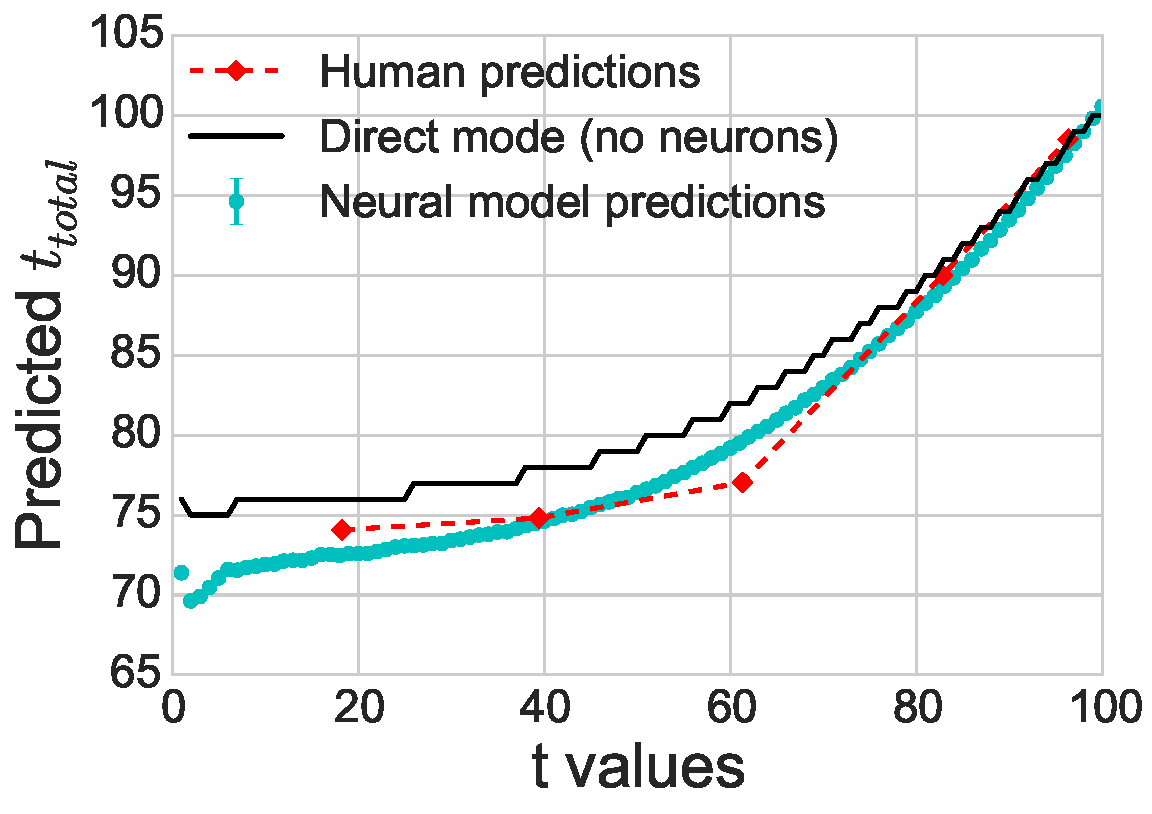
\includegraphics[width=80mm, keepaspectratio]{nengo_predictions.pdf}
\end{center}
\caption{Inference results from neural model (95\% confidence intervals), compared to humans and Direct mode - our model with computations in low-dimensional (20 dimensional basis) space, but without neurons.}
\label{fig:nengo_predictions}
\end{figure}

\begin{figure*}[h]
    \centering
    \begin{subfigure}{.43\textwidth}
        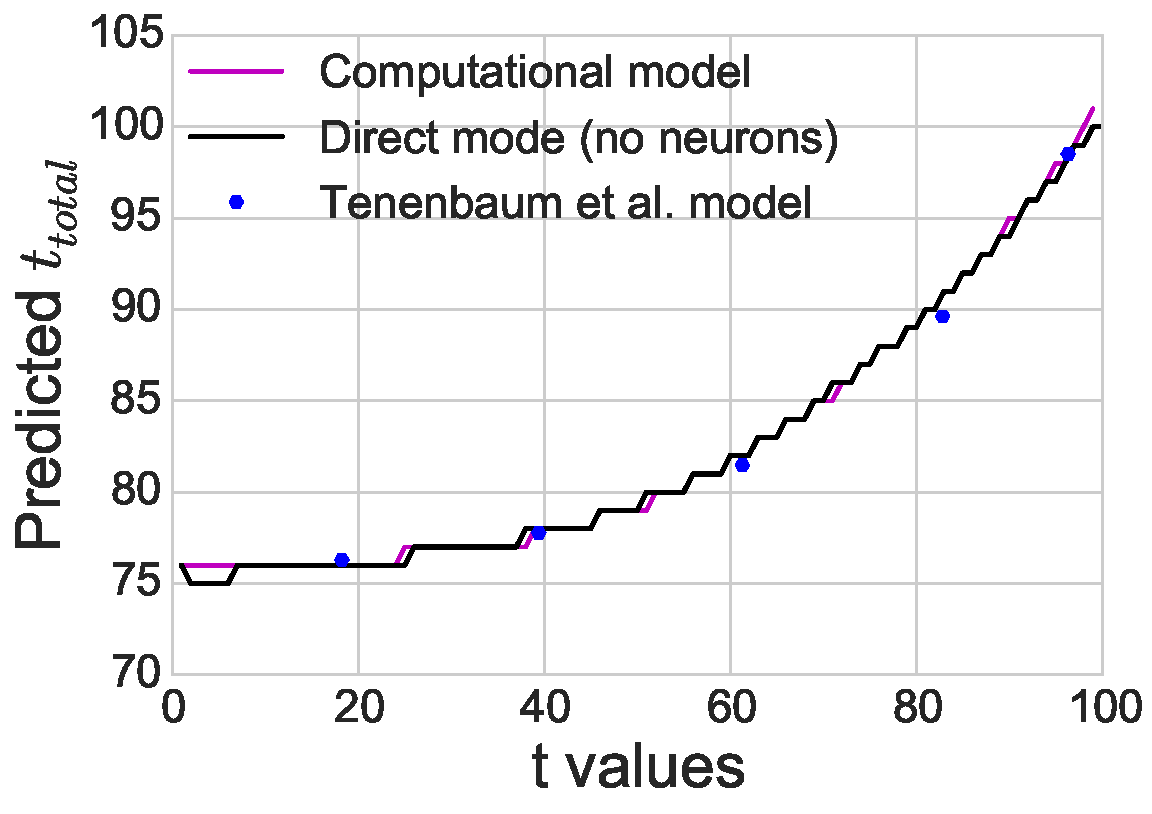
\includegraphics[width=\linewidth]{replication}
        \caption{No error due to low dimensional embedding.} 
        \label{fig:replication}
    \end{subfigure}
    \begin{subfigure}{.43\textwidth}
        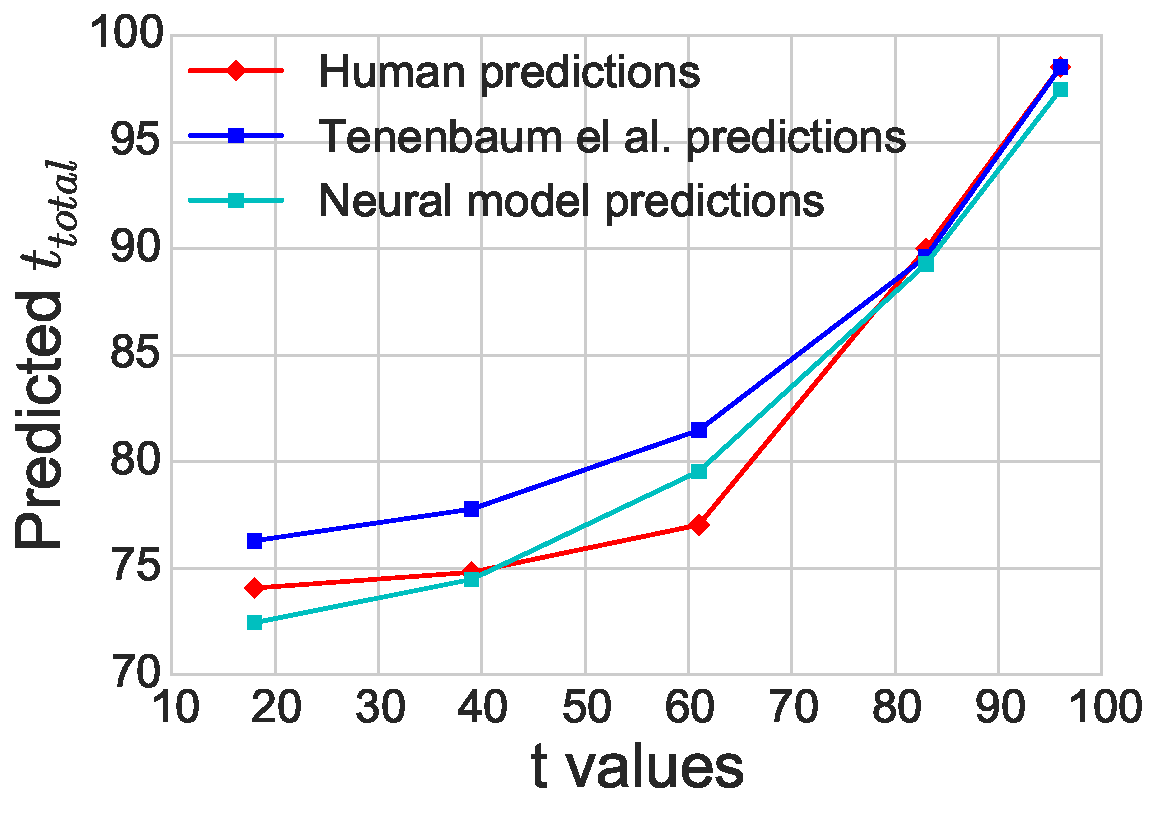
\includegraphics[width=\linewidth]{kolmogrov_results}
        \caption{Data used for the goodness of fit test.} 
        \label{fig:kolmogrov_results}
    \end{subfigure}
    \caption{(a) Results from~\citeA{griffiths2006optimal} model  (only data corresponding to human data), Computational model i.e., our replication of their model, and Direct mode i.e., our model with computations in low-dimensional space, but without neurons. (b) Kolmogorov-Smirnov (K-S) test results. Dissimilarity relative to human predictions -~\citeA{griffiths2006optimal} model: 9.628, neural model: 1.959. Neural model and human data are median predictions. Note:~\citeA{griffiths2006optimal} model data and human data were obtained from Figure~\ref{fig:model_prior_prediction}B through a web plot digitizer.
    }\label{fig:model_comparison}
\end{figure*}


%\subsection{Results}
Figure~\ref{fig:nengo_predictions} shows the inference results obtained from the spiking neural network run in the Nengo~\cite{bekolay2014nengo} software package. Model predictions are plotted for current ages ($t$) from 1 to 100. The difference between the results in Direct mode and Neuron mode is due to the limited number of neurons in the \textit{Normalized Posterior} ensemble. As the number of neurons in this ensemble increases, the results approach the Direct mode results (800 neurons provide the best fit to human data). Thus, neural results match the human data better due to the approximate representation of the normalized posterior by the neurons in the \textit{Normalized Posterior} ensemble. The tuning curves of the neurons in this ensemble were fit to a function space consisting of a family of distributions which have three parameters (similar to the parameters in the prior) and also depend on the current age ($t$) (similar to the likelihood function). The three parameters: \textit{a} - the skewness parameter was varied from -7 to -4, \textit{scale} - used to scale the distribution was varied from 26 to 29 and \textit{loc} - used to shift the distribution was varied between 49 to 101. The current age ($t$) was varied in the range of +/-5 for a given age in a trial except ages below 5 for which the range was taken to be from [1, 10]. This provides the function space that was used to sample the encoders for \textit{Normalized Posterior} ensemble. 

We use the Kolmogorov-Smirnov (K-S) test to examine the goodness of fit of the neural model predictions relative to the ~\citeA{griffiths2006optimal} model. The data used for the K-S test are shown in Figure~\ref{fig:kolmogrov_results}. The dissimilarity of the~\citeA{griffiths2006optimal} model relative to human predictions is 9.628, while that of the neural model is 1.959, indicating the much closer fit of the neural model to the human data. Figure~\ref{fig:replication} shows a comparison between the~\citeA{griffiths2006optimal} model, the computational model (our replication of their model), and direct mode (our model with computations in a compressed 20 dimensional space, but without neurons). Since the results obtained from the direct mode are the same as the computational model, the low dimensional embedding is not losing any information. However, we expect some error due to this constraint for more complex priors (though we have not explored the minimum dimensionality for this prior). 

Overall, our results suggest that the closer fit of the neural data can be solely attributed to fitting the neuron tuning curves in the \textit{Normalized Posterior} ensemble, where 800 neurons provide the best match to human performance. Since the low-dimensional neural implementation can be made to match the human data, this is some evidence in support of the hypothesis that human brains represent low-dimensional state spaces (low-dimensional parameterizations of high-dimensional distributions fit using neural tuning curves).

\section{Generalized life span inference}

In our neural model, we use the prior obtained empirically by~\citeA{griffiths2006optimal}. However, our neural modeling methods can further be used to explore how this prior might be learned in the human brain. Here, we lay some theoretical ground work for addressing this question, while building the complete neural model remains for future work.

We assume that priors that humans have about life spans are a result of their experiences encountering people of different ages in their daily lives. Thus the prior will be inferred from the data that comes from daily experience. We further assume that the prior is parameterized by some unknown hyperparameters ($\alpha$) which are to be estimated from the observed ages of $n$ distinct people, given by $\vec{X} = \{x_1, \ldots, x_n\}$. Here, each random variable $x_i$ corresponds to a separate $t$ from the previous model. Likewise, we model each element of $\vec{X}$ as being drawn independently from each element of $\vec{Z} = \{z_1, \ldots, z_n\}$ corresponding to the (unknown or hidden) life spans of these same $n$ people. Each random variable $z_i$ corresponds to a separate $t_{total}$ from the previous model, which in turn is drawn from the unknown prior. We now describe two standard methods for determining a prior by obtaining an estimate $\hat{\alpha}$ of the hyperparameters.

If we do not know the actual prior, then the optimal solution can be found by trying them all. That is, we directly find the hyperparameters $\hat{\alpha}$ that maximize the marginal likelihood of the observed data, $L(\alpha; \vec{X})$ (or equivalently the log-likelihood for numerical stability):
\begin{equation}
\label{eqn:marg_likelihood}
\begin{aligned}
%L(\alpha; \vec{X}) &= p(\vec{X} | \alpha) = \prod_{i=1}^n p(x_i | \alpha) = \prod_{i=1}^n \sum_{z_i} p(x_i, z_i | \alpha) \\
%\implies \: 
\hat{\alpha} &= \text{argmax}_\alpha L(\alpha; \vec{X})
% && &= \text{argmax}_\alpha \log L(\alpha; \vec{X}) \\
= \text{argmax}_\alpha \sum_{i=1}^n \log \sum_{z_i} p(x_i, z_i | \alpha) .
\end{aligned}
\end{equation}
In general, however, the procedure described above is intractable, since it requires that we iterate over all combinations of $\alpha$ and $\vec{Z}$. This motivates near-optimal iterative procedures such as the widely-used expectation maximization algorithm~\cite<EM;>{dempster1977maximum}.
Below we work out the details of the EM procedure for the case where the hyperparameters are $\alpha = (\mu, \sigma^2)$, i.e., the prior is assumed to be normally distributed with unknown moments. We begin by simplifying the expectation function using independence and other known facts about the model:
\begin{equation}
\begin{aligned}
Q(\alpha | \alpha^{(t)}) &= E_{\vec{Z}|\vec{X},\alpha^{(t)}} \left[ \log L(\alpha; \vec{X}, \vec{Z}) \right] \\
&= \sum_{i=1}^n E_{z_i|x_i,\alpha^{(t)}} \left[ \log L(\alpha; x_i, z_i) \right] \\
%&= \sum_{i=1}^n \sum_{z_i} p(z_i | x_i, \alpha^{(t)}) \log p(x_i, z_i | \alpha) \\
% &= \sum_{i=1}^n \sum_{z_i} T(x_i, z_i) \log \left( p(x_i | z_i) p(z_i | \alpha) \right) \\
&= \sum_{i=1}^n \sum_{z_i} T(x_i, z_i) \log \left( p(z_i | \alpha) / z_i \right) ,
\end{aligned}
\end{equation}
where we have defined $T(x_i, z_i) := p(z_i | x_i, \alpha^{(t)})$ to be some fixed function with respect to $\alpha^{(t)}$.
% $p(x_i, z_i | \alpha) = p(x_i | z_i) p(z_i | \alpha)$, with $\alpha^{(t)}$ included, since $p(x_i | z_i, \alpha) = p(x_i | z_i)$ by assumption.
% Substituting $p(x_i | z_i) = 1 / z_i$ for all $z_i$ is okay since $T(x_i, z_i) = 0$ for $z_i \le x_i$ by definition.
Next, we simplify the log expression using our model of the prior:  %, with unknown $\alpha = (\mu, \sigma)$:
\begin{equation}
\begin{aligned}
\log \left( p(z_i | \alpha) / z_i \right) = \log \left( \frac{1}{\sqrt{2\sigma^2 \pi}} e^{-\frac{(z_i - \mu)^2}{2\sigma^2}} \right) - \log z_i \\
= -\frac{1}{2} \left( (z_i - \mu)^2 / \sigma^2 + \log \sigma^2 + \log \left( 2\pi \right) + 2 \log z_i \right) ,
\end{aligned}
\end{equation}
and then differentiate this with respect to $\mu$:
\begin{equation}
\begin{aligned}
\frac{\partial \log \left( p(z_i | \alpha) / z_i \right)}{\partial \mu} &= (z_i - \mu)\sigma^2 ,
\end{aligned}
\end{equation}
and with respect to $\sigma^2$:
\begin{equation}
\begin{aligned}
\frac{\partial \log \left( p(z_i | \alpha) / z_i \right)}{\partial \sigma^2} %&= \frac{1}{2}(z_i - \mu)^2/\sigma^4 - \frac{1}{2}/\sigma^2
= \frac{1}{2}\left((z_i - \mu)^2 - \sigma^2 \right)/\sigma^4 .
\end{aligned}
\end{equation}
By linearity of differentiation, we then know that the derivatives of $Q(\cdot)$ are zero when:
\begin{equation}
\begin{aligned}
\frac{\partial Q(\alpha | \alpha^{(t)})}{d \mu} &= \sum_{i=1}^n \sum_{z_i} T(x_i, z_i) (z_i - \mu)\sigma^2 = 0  \\
\iff \quad \mu &= \frac{\sum_{i=1}^n \sum_{z_i} z_i T(x_i, z_i)}{\sum_{i=1}^n \sum_{z_i} T(x_i, z_i)} ,  \hspace{0.3cm}\text{and similarly:}
\end{aligned}
\end{equation}
%and similarly:
\begin{equation}
\begin{aligned}
\frac{\partial Q(\alpha | \alpha^{(t)})}{d \sigma^2} &= \sum_{i=1}^n \sum_{z_i} T(x_i, z_i) \frac{1}{2}\left((z_i - \mu)^2 - \sigma^2 \right)/\sigma^4 = 0  \\
\iff \quad \sigma^2 &= \frac{\sum_{i=1}^n \sum_{z_i} (z_i - \mu)^2 T(x_i, z_i)}{\sum_{i=1}^n \sum_{z_i} T(x_i, z_i)} .
\end{aligned}
\end{equation}
Finally, by the generalized Bayes' rule, we know:
$$
T(x_i, z_i) = p(z_i | x_i, \alpha^{(t)}) = \frac{p(z_i, x_i | \alpha^{(t)})}{ \sum_{z_i} p(z_i, x_i | \alpha^{(t)}) } ,
$$
which we may compute via Eq.~\ref{eqn:bayes_rule}.
We also note that since $T(\cdot)$ is a probability density function over $z_i$, that:
$$
\sum_{i=1}^n \sum_{z_i} T(x_i, z_i) = \sum_{i=1}^n 1 = n .
$$
Therefore, each EM iteration must make the update $\alpha^{(t+1)} = (\mu^{(t+1)}, \sigma^{(t+1)})$, where:
\begin{equation}
\begin{aligned}
\mu^{(t+1)} &= \frac{1}{n} \sum_{i=1}^n \frac{\sum_{z_i} z_i p(z_i, x_i | \alpha^{(t)})}{\sum_{z_i} p(z_i, x_i | \alpha^{(t)})} \\
\sigma^{(t+1)} &= \sqrt{\frac{1}{n}  \sum_{i=1}^n \frac{\sum_{z_i} (z_i - \mu^{(t+1)})^2 p(z_i, x_i | \alpha^{(t)})}{\sum_{z_i} p(z_i, x_i | \alpha^{(t)})}} .
\end{aligned}
\end{equation}
This converges to some locally optimal estimate of the hyperparameters. For initial $\alpha^{(0)}$ chosen sufficiently close to global optimum $\hat{\alpha}$ given by Eq.~\ref{eqn:marg_likelihood}, this converges to the optimum.

This provides a tractable procedure for updating the prior. In particular, we begin with some initial guess at the hyperparameters, and then update them iteratively to better explain the observed data. In practice only a few iterations are required (results not shown). Once we have an estimate of the hyperparameters ($\hat{\alpha}$), we then know the prior $p(t_{total} | \hat{\alpha})$. This prior can be used directly by the previously described model to provide a good prediction. In fact, it is possible to run both the prior optimization and inference at the same time, and both will become progressively more accurate over time.

\section{Conclusions}

We have presented a spiking neural network able to effectively perform Bayesian inference in a manner that more accurately matches human behavior than an ideal Bayesian computation.  We constructed the network using the NEF to map function spaces into vector spaces and approximate the necessary computations.  We suggested a means of estimating the prior for the life span task that can be implemented using these same methods. 
\newline \textbf{Notes} \hspace{0.3cm} Supplemental material (scripts and derivations) can be found at https://github.com/ctn-waterloo/cogsci17-infer.

\section{Acknowledgments}
This work was supported by CFI and OIT infrastructure funding, the Canada Research Chairs program, NSERC Discovery grant 261453, ONR grant N000141310419, AFOSR grant FA8655-13-1-3084, OGS, and NSERC CGS-D.

\bibliographystyle{apacite}

\setlength{\bibleftmargin}{.125in}
\setlength{\bibindent}{-\bibleftmargin}

\bibliography{CogSci_Template}


\end{document}
